\documentclass{exam}

\usepackage{siunitx} 
\usepackage{graphicx}
\usepackage[fleqn]{amsmath}
\usepackage{cancel}
\usepackage{float}
\usepackage{mdwlist}
\usepackage{booktabs}
\usepackage{cancel}
\usepackage{polynom}
\usepackage{caption}
\usepackage{fullpage}
\usepackage{comment}
\usepackage{enumerate}

\newcommand{\degree}{\ensuremath{^\circ}} 
\everymath{\displaystyle}

% \begin{figure}[H]
%   \centering
%   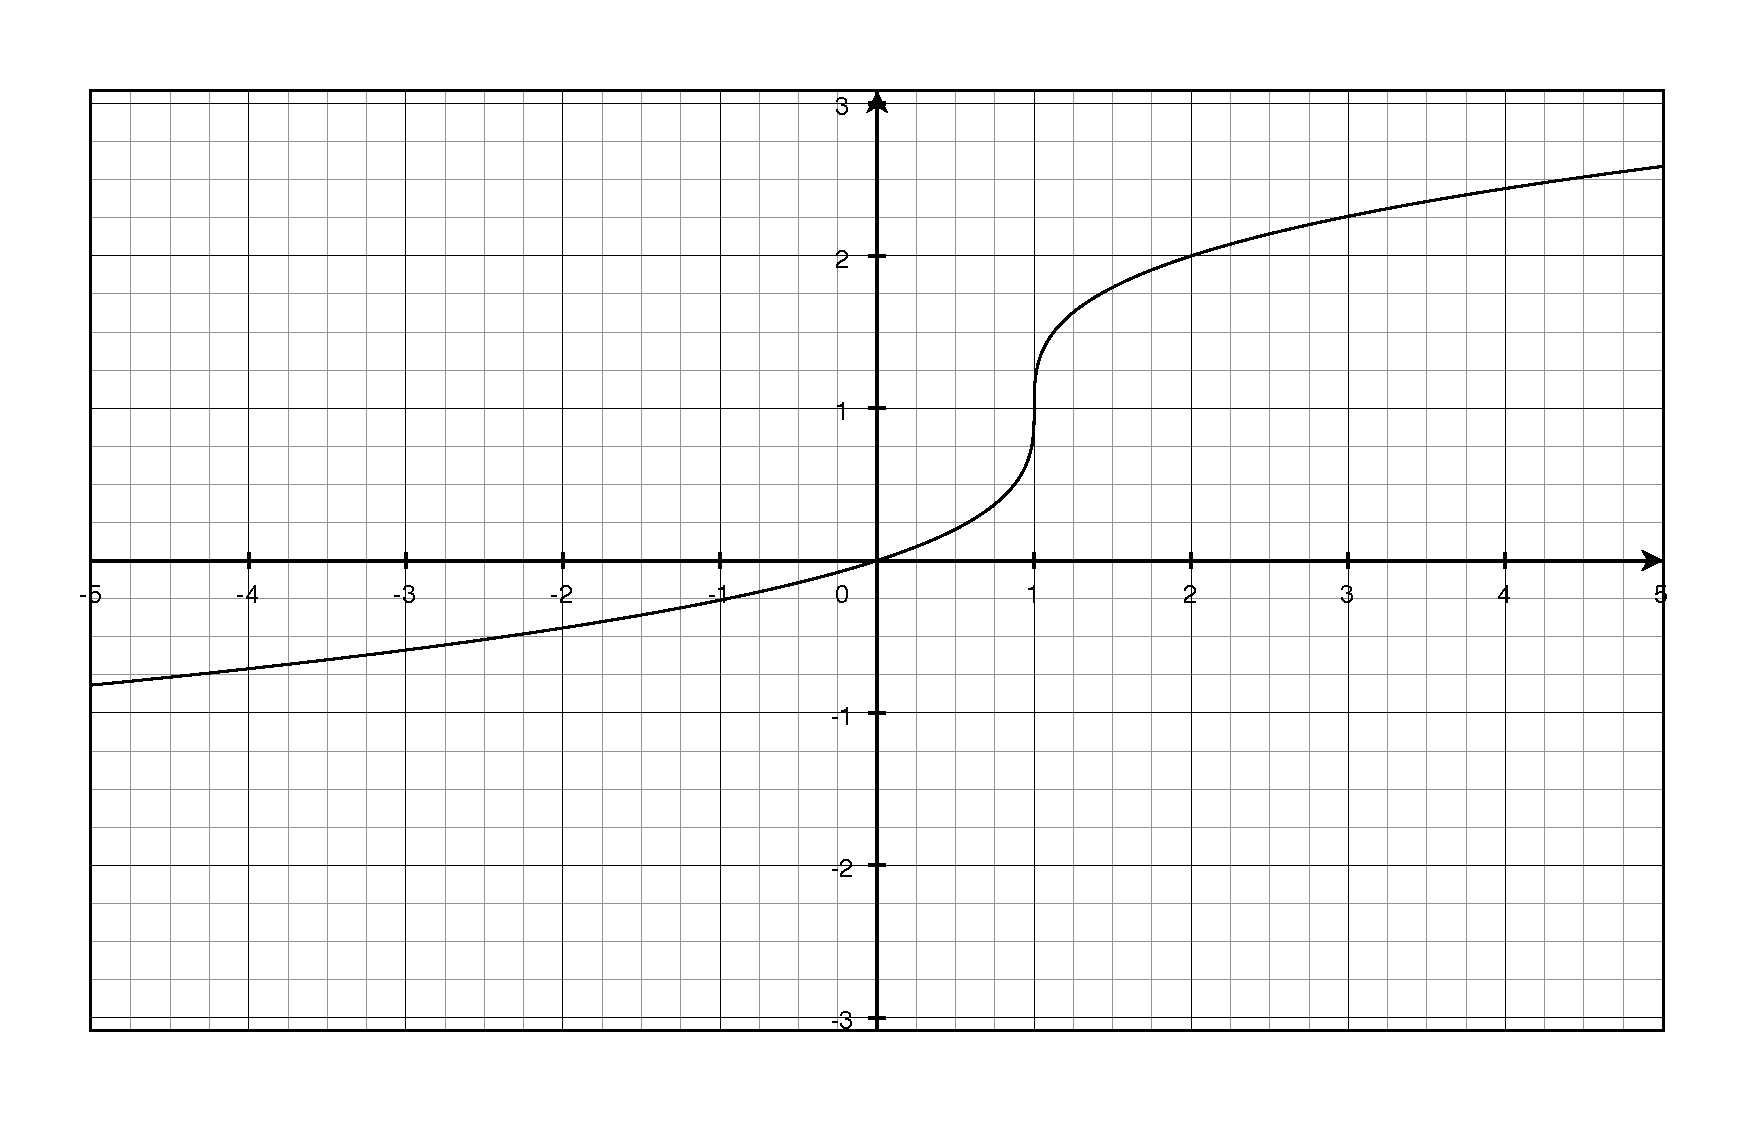
\includegraphics[scale=.3]{question7.eps}
%   \caption*{question 7}
% \end{figure}

% \begin{tabular}{cc}
%   \toprule
%   period & amplitude \\
%   \midrule
%     $\pi$ & $2$ \\
%   \bottomrule
% \end{tabular}

\printanswers
\excludecomment{comment}

\ifprintanswers 
  \usepackage{2in1, lscape} 
\fi

\author{}
\date{\today}
\title{Math 142 \\ Homework Three}

\begin{document}

  \maketitle

  \section{Homework}
  Section 5.3: 

  \section{Extra Credit}
  TO DO

  \ifprintanswers
    \section{Section 5.3}
    \begin{description}

      \item[1]
        \begin{figure}[H]
          \centering
          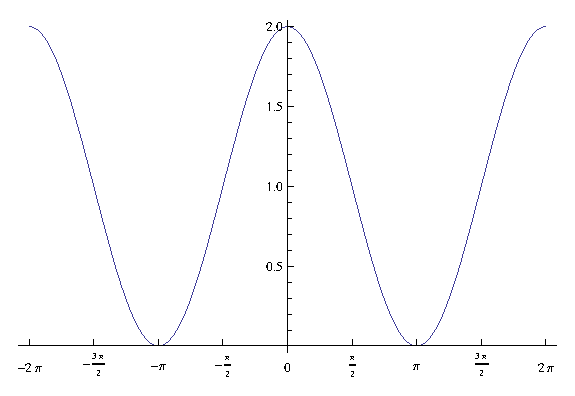
\includegraphics[scale=0.8]{exercise01.eps}
          \caption{$f(x) = 1 + \cos x$}
        \end{figure}

      \item[2]
        \begin{figure}[H]
          \centering
          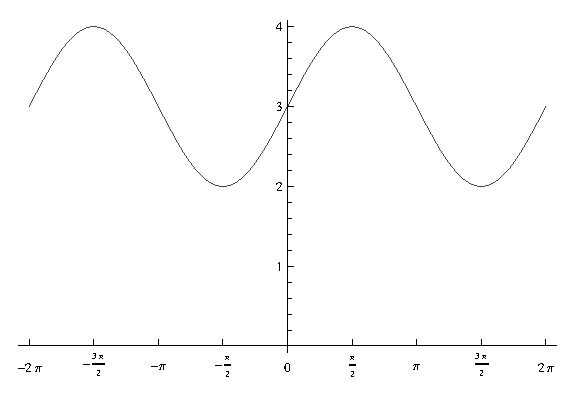
\includegraphics[scale=0.8]{exercise02.eps}
          \caption{$f(x) = 3 + \sin x$}
        \end{figure}

      \item[3]
        \begin{figure}[H]
          \centering
          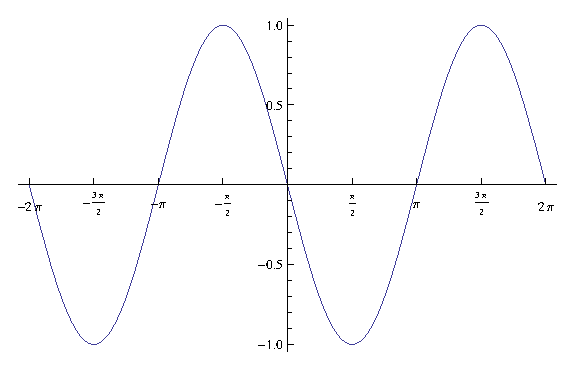
\includegraphics[scale=0.8]{exercise03.eps}
          \caption{$f(x) = -\sin x$}
        \end{figure}

      \item[4]
        \begin{figure}[H]
          \centering
          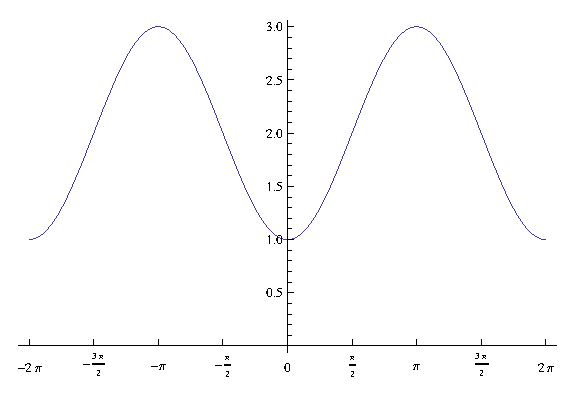
\includegraphics[scale=0.8]{exercise04.eps}
          \caption{$f(x) = 2 - \cos x$}
        \end{figure}

      \item[5]
        \begin{figure}[H]
          \centering
          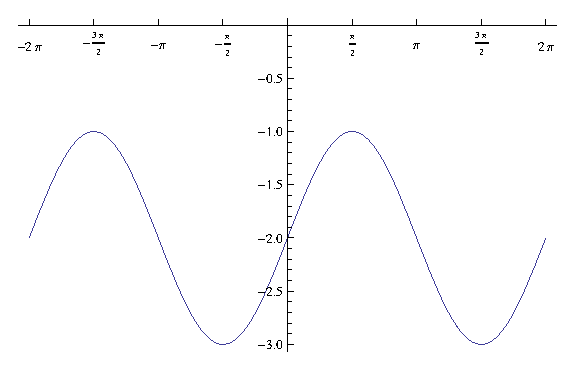
\includegraphics[scale=0.8]{exercise05.eps}
          \caption{$f(x) = -2 + \sin x$}
        \end{figure}

      % \item[6]
      %   \begin{figure}[H]
      %     \centering
      %     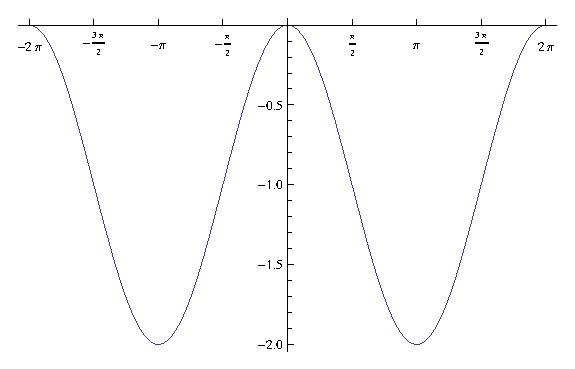
\includegraphics[scale=0.8]{exercise06.eps}
      %     \caption{$f(x) = -1 + \cos x$}
      %   \end{figure}

      % \item[7]
      %   \begin{figure}[H]
      %     \centering
      %     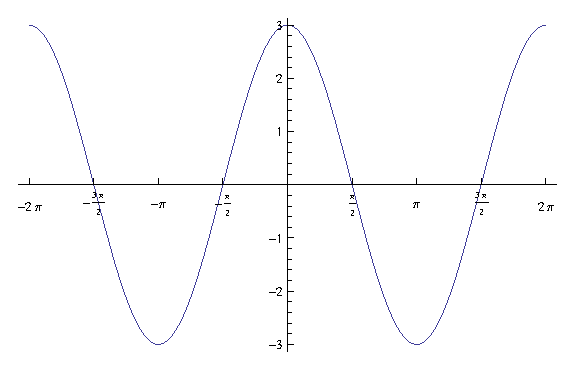
\includegraphics[scale=0.8]{exercise07.eps}
      %     \caption{$g(x) = 3 \cos x$}
      %   \end{figure}

      % \item[8]
      %   \begin{figure}[H]
      %     \centering
      %     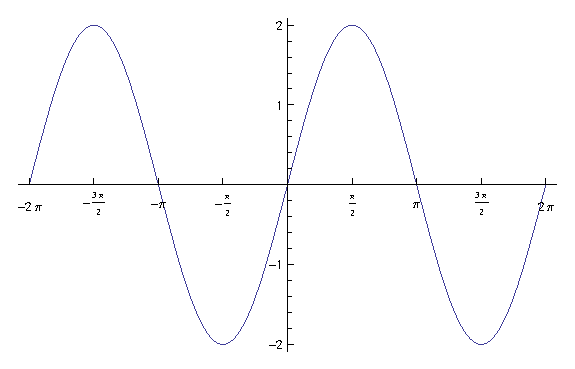
\includegraphics[scale=0.8]{exercise08.eps}
      %     \caption{$g(x) = 2 \sin x$}
      %   \end{figure}

      % \item[9]
      %   \begin{figure}[H]
      %     \centering
      %     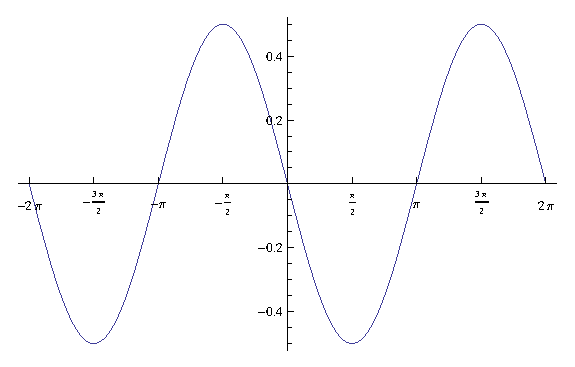
\includegraphics[scale=0.9]{exercise09.eps}
      %     \caption{$g(x) = - \frac{1}{2} \sin x$}
      %   \end{figure}

      \item[10]
        \begin{figure}[H]
          \centering
          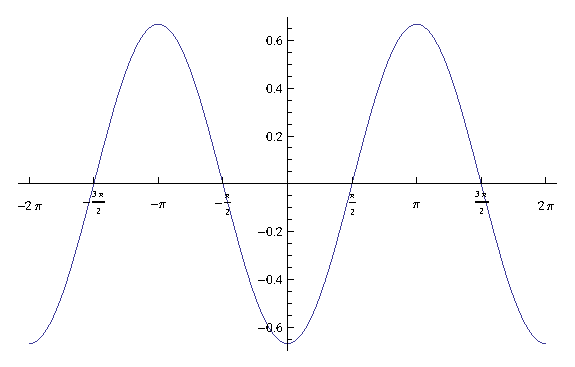
\includegraphics[scale=0.9]{exercise10.eps}
          \caption{$g(x) = - \frac{2}{3} \cos x$}
        \end{figure}

      \item[11]
        \begin{figure}[H]
          \centering
          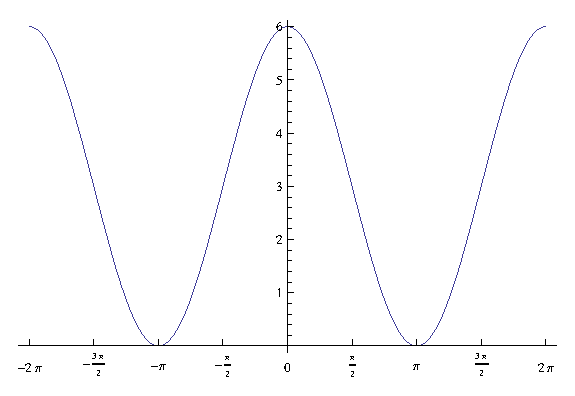
\includegraphics[scale=0.9]{exercise11.eps}
          \caption{$g(x) = 3 + 3 \cos x$}
        \end{figure}

      \item[12]
        \begin{figure}[H]
          \centering
          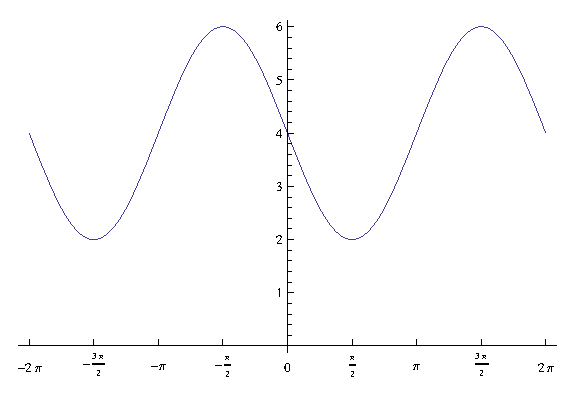
\includegraphics[scale=0.9]{exercise12.eps}
          \caption{$g(x) = 4 - 2 \sin x$}
        \end{figure}

      \item[13]
        \begin{figure}[H]
          \centering
          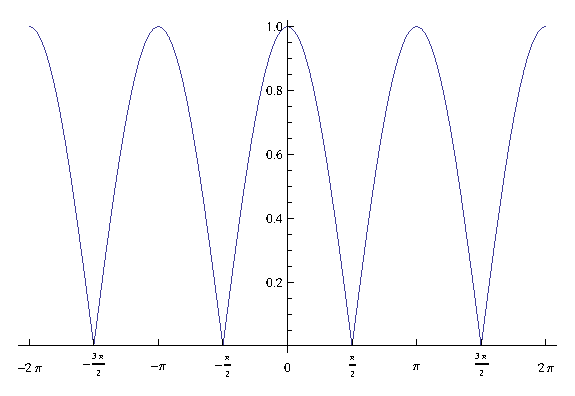
\includegraphics[scale=0.9]{exercise13.eps}
          \caption{$h(x) = | \cos x |$}
        \end{figure}

      \item[14]
        \begin{figure}[H]
          \centering
          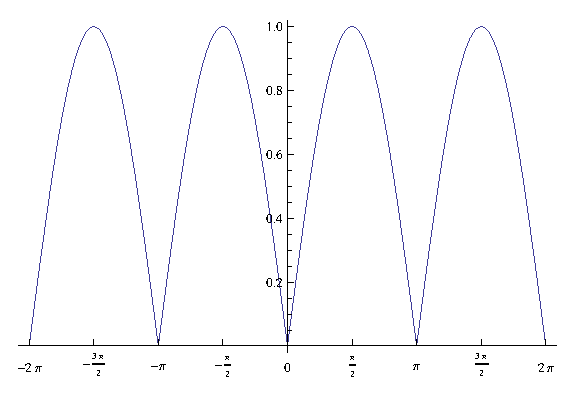
\includegraphics[scale=0.9]{exercise14.eps}
          \caption{$h(x) = | \sin x |$}
        \end{figure}

      \item[15]
        \begin{figure}[H]
          \centering
          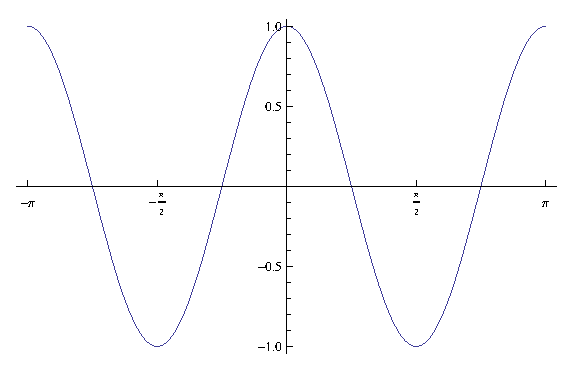
\includegraphics[scale=0.8]{exercise15.eps}
          \caption{$y = \cos 2x$}
        \end{figure}

        \begin{tabular}[H]{lr}
          \toprule
          amplitude & 1 \\
          period & $\pi$ \\
          \bottomrule
        \end{tabular}

      \item[16]
        \begin{figure}[H]
          \centering
          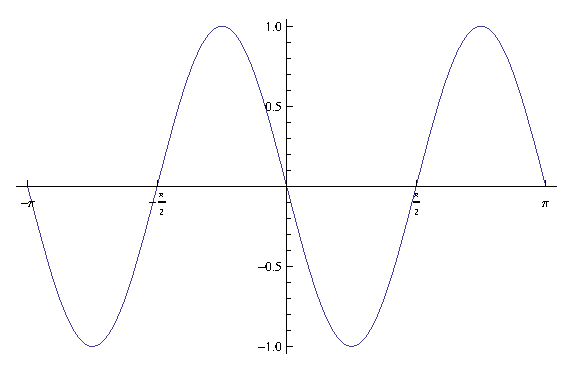
\includegraphics[scale=0.9]{exercise16.eps}
          \caption{$y = - \sin 2x$}
        \end{figure}

        \begin{tabular}[H]{lr}
          \toprule
          amplitude & -1 \\
          period & $\pi$ \\
          \bottomrule
        \end{tabular}

      \item[17]
        \begin{figure}[H]
          \centering
          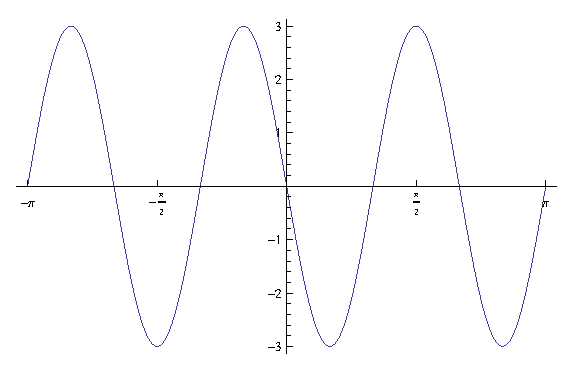
\includegraphics[scale=0.9]{exercise17.eps}
          \caption{$y = - 3 \sin 3x$}
        \end{figure}

        \begin{tabular}[H]{lr}
          \toprule
          amplitude & $-3$ \\
          period & $\frac{3 \pi}{2}$ \\
          \bottomrule
        \end{tabular}

      \item[18]
        \begin{figure}[H]
          \centering
          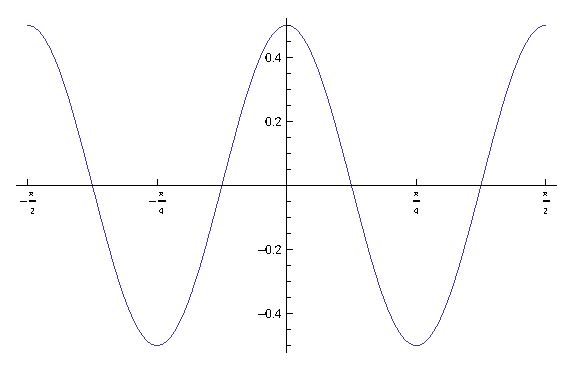
\includegraphics[scale=0.9]{exercise18.eps}
          \caption{$y = \frac{1}{2} \cos 4x$}
        \end{figure}

        \begin{tabular}[H]{lr}
          \toprule
          amplitude & $\frac{1}{2}$ \\
          \midrule
          period & $\frac{\pi}{4}$ \\
          \bottomrule
        \end{tabular}

      \item[23]
        \begin{figure}[H]
          \centering
          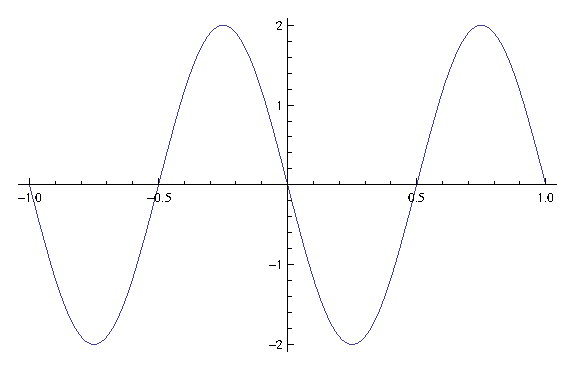
\includegraphics[scale=0.9]{exercise23.eps}
          \caption{$y = -2 \sin 2 \pi x$}
        \end{figure}

        \begin{tabular}[H]{lr}
          \toprule
          amplitude & $-2$ \\
          \midrule
          period & $1$ \\
          \bottomrule
        \end{tabular}

      \item[24]
        \begin{figure}[H]
          \centering
          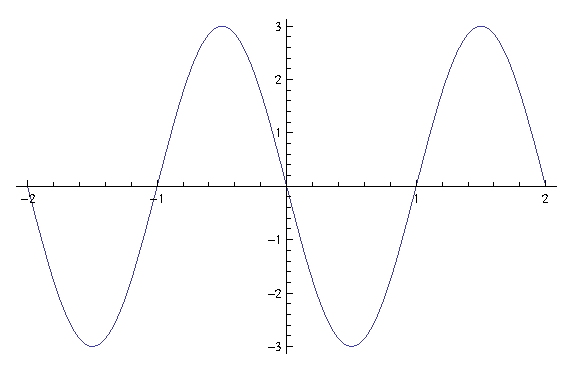
\includegraphics[scale=0.9]{exercise24.eps}
          \caption{$y = -3 \sin \pi x$}
        \end{figure}

        \begin{tabular}[H]{lr}
          \toprule
          amplitude & $-3$ \\
          \midrule
          period & $2$ \\
          \bottomrule
        \end{tabular}

      \item[25]
        \begin{figure}[H]
          \centering
          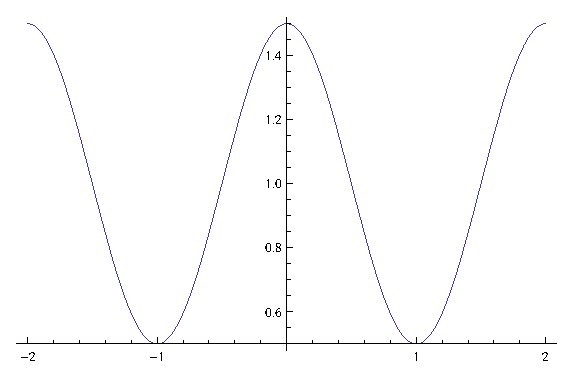
\includegraphics[scale=0.9]{exercise25.eps}
          \caption{$y = 1 + \frac{1}{2} \cos \pi x$}
        \end{figure}

        \begin{tabular}[H]{lr}
          \toprule
          amplitude & $\frac{1}{2}$ \\
          \midrule
          period & $2$ \\
          \bottomrule
        \end{tabular}

      \item[26]
        \begin{figure}[H]
          \centering
          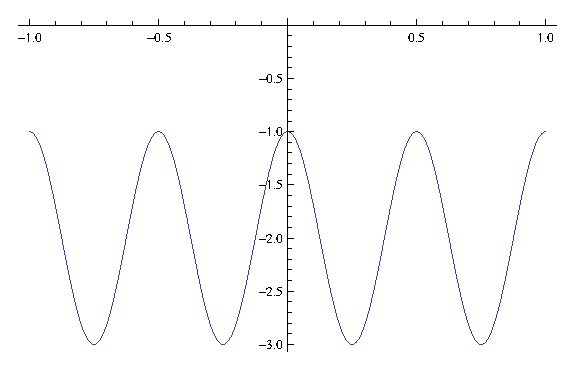
\includegraphics[scale=0.9]{exercise26.eps}
          \caption{$y = -2 + \cos 4 \pi x$}
        \end{figure}

        \begin{tabular}[H]{lr}
          \toprule
          amplitude & $1$ \\
          \midrule
          period & $\frac{1}{2}$ \\
          \bottomrule
        \end{tabular}

      \item[27]
        \begin{figure}[H]
          \centering
          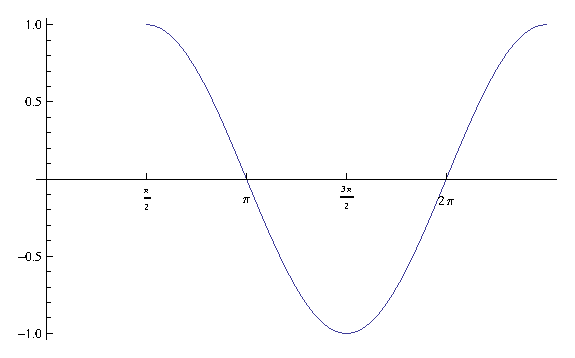
\includegraphics[scale=0.8]{exercise27.eps}
          \caption{$y = \cos \left( x - \frac{\pi}{2} \right)$}
        \end{figure}

        \begin{tabular}[H]{lr}
          \toprule
          amplitude & $1$ \\
          \midrule
          period & $2 \pi$ \\
          \midrule
          phase shift & $\frac{\pi}{2}$ \\
          \bottomrule
        \end{tabular}

      \item[28]
        \begin{figure}[H]
          \centering
          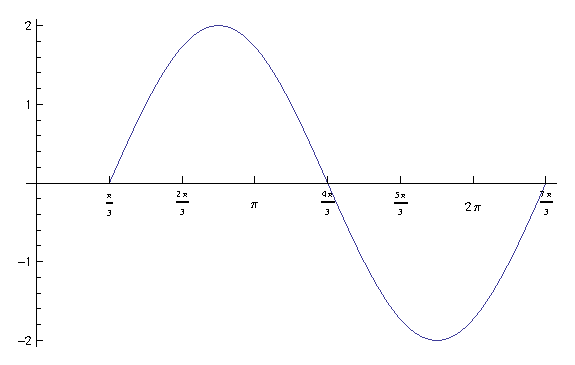
\includegraphics[scale=0.8]{exercise28.eps}
          \caption{$y = 2 \sin \left( x - \frac{\pi}{3} \right)$}
        \end{figure}

        \begin{tabular}[H]{lr}
          \toprule
          amplitude & $2$ \\
          \midrule
          period & $2 \pi$ \\
          \midrule
          phase shift & $\frac{\pi}{3}$ \\
          \bottomrule
        \end{tabular}

      \item[29]
        \begin{figure}[H]
          \centering
          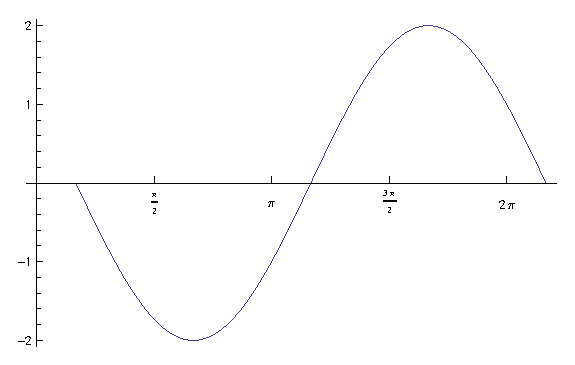
\includegraphics[scale=0.8]{exercise29.eps}
          \caption{$y = - 2 \sin \left( x - \frac{\pi}{6} \right)$}
        \end{figure}

        \begin{tabular}[H]{lr}
          \toprule
          amplitude & $-2$ \\
          \midrule
          period & $2 \pi$ \\
          \midrule
          phase shift & $\frac{\pi}{6}$ \\
          \bottomrule
        \end{tabular}

      \item[30]
        \begin{figure}[H]
          \centering
          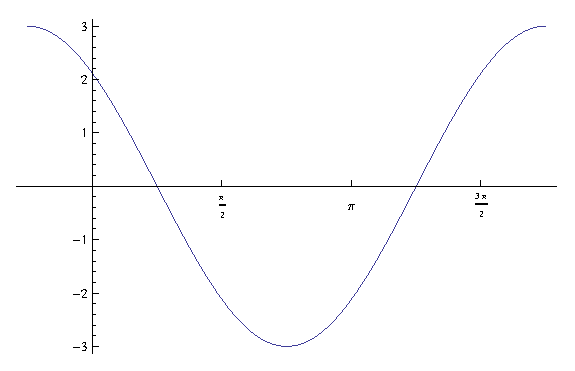
\includegraphics[scale=0.8]{exercise30.eps}
          \caption{$y = 3 \cos \left( x + \frac{\pi}{4} \right)$}
        \end{figure}

        \begin{tabular}[H]{lr}
          \toprule
          amplitude & $3$ \\
          \midrule
          period & $2 \pi$ \\
          \midrule
          phase shift & $\frac{\pi}{4}$ \\
          \bottomrule
        \end{tabular}

      \item[31]
        \begin{figure}[H]
          \centering
          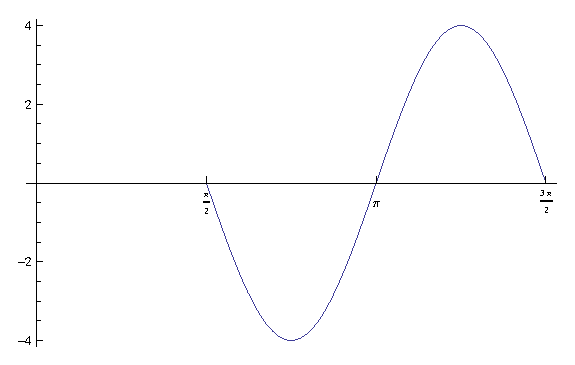
\includegraphics[scale=0.8]{exercise31.eps}
          \caption{$y = -4 \sin 2 \left( x + \frac{\pi}{2} \right)$}
        \end{figure}

        \begin{tabular}[H]{lr}
          \toprule
          amplitude & $-4$ \\
          \midrule
          period & $\pi$ \\
          \midrule
          phase shift & $\pi$ \\
          \bottomrule
        \end{tabular}

      \item[32]
        \begin{figure}[H]
          \centering
          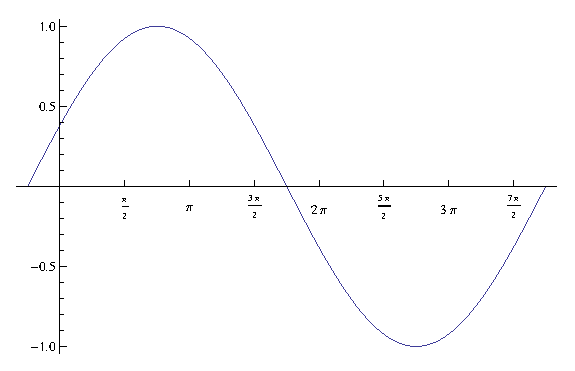
\includegraphics[scale=0.8]{exercise32.eps}
          \caption{$y = \sin \frac{1}{2} \left( x + \frac{\pi}{4} \right)$}
        \end{figure}

        \begin{tabular}[H]{lr}
          \toprule
          amplitude & $\frac{1}{2}$ \\
          \midrule
          period & $4 \pi$ \\
          \midrule
          phase shift & $- \frac{\pi}{4}$ \\
          \bottomrule
        \end{tabular}

      \item[33]
        \[
          y = 5 \cos \left( 3x - \frac{\pi}{4} \right) = 5 \cos 3 \left( x - \frac{\pi}{12} \right)
        \]

        \begin{figure}[H]
          \centering
          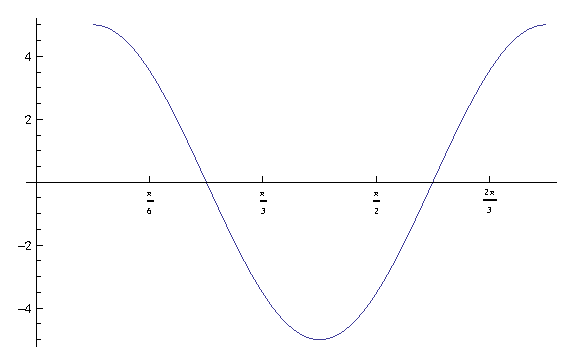
\includegraphics[scale=0.8]{exercise33.eps}
          \caption{$y = 5 \cos \left( 3x - \frac{\pi}{4} \right)$}
        \end{figure}

        \begin{tabular}[H]{lr}
          \toprule
          amplitude & $5$ \\
          \midrule
          period & $\frac{2 \pi}{3}$ \\
          \midrule
          phase shift & $- \frac{\pi}{12}$ \\
          \bottomrule
        \end{tabular}

      \pagebreak

      \item[34]
        \[
          y = 2 \sin \left( \frac{2}{3} x - \frac{\pi}{6} \right) = 2 \sin \frac{2}{3} \left( x - \frac{\pi}{4} \right)
        \]

        \begin{figure}[H]
          \centering
          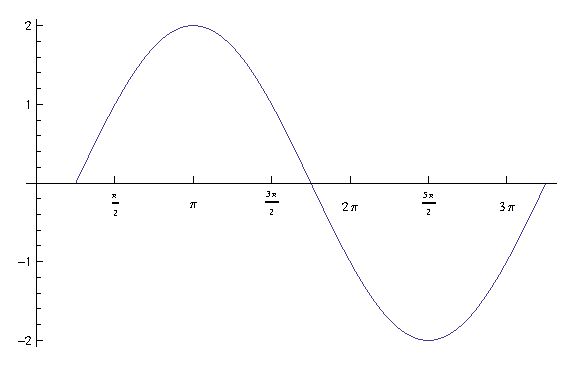
\includegraphics[scale=1.0]{exercise34.eps}
          \caption{$y = 2 \sin \left( \frac{2}{3} x - \frac{\pi}{6} \right)$}
        \end{figure}

        \begin{tabular}[H]{lr}
          \toprule
          amplitude & $2$ \\
          \midrule
          period & $3 \pi$ \\
          \midrule
          phase shift & $\frac{\pi}{4}$ \\
          \bottomrule
        \end{tabular}

      \pagebreak

      \item[35]
        \[
          y = \frac{1}{2} - \frac{1}{2} \cos \left( 2x - \frac{\pi}{3} \right) = \frac{1}{2} \cos 2 \left( x - \frac{\pi}{6} \right)
        \]

        \begin{figure}[H]
          \centering
          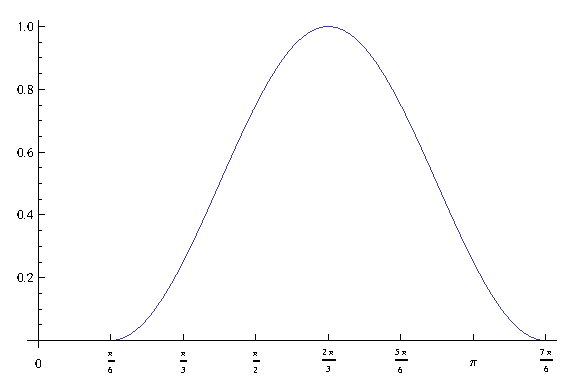
\includegraphics[scale=1.0]{exercise35.eps}
          \caption{$y = \frac{1}{2} - \frac{1}{2} \cos \left( 2x - \frac{\pi}{3} \right)$}
        \end{figure}

        \begin{tabular}[H]{lr}
          \toprule
          amplitude & $- \frac{1}{2}$ \\
          \midrule
          period & $\pi$ \\
          \midrule
          phase shift & $\frac{\pi}{6}$ \\
          \bottomrule
        \end{tabular}

    \end{description}
  \else
    \vspace{1 cm}
    \begin{quote}
      \begin{em}
        TO DO
      \end{em}
    \end{quote}
    \hspace{1 cm} --Shunryu Suzuki
  \fi

\end{document}

